%\chapter{System design}

%In this chapter, design of the radio link and component selection are described. During the design process, multiple iteration of component selection, validation and link budget calculation were made, this chapter describes the final result of the design.

\chapter{System requirements}
\section{Communication sessions}
PW-Sat2 was designed to be deployed on \SI{600}{\kilo\meter}, Sun-synchronous, polar orbit. Due to the Earts rotation, ground station coverage is bounded, and communication with the satellite is limited to communication session during satellite overpass.

Simulations performed using Gpredict software \cite{gpredict_website} shown that communication sessions will happen \si{5}-\si{6} times per day, \si{5}-\SI{10}{\minute} each. This summarizes to the total communication time to average \SI{30}{\minute} per day. Typical radio coverage of the satellite is shown in the figure \ref{gpredict_pass}.

\begin{figure}
    \centering
    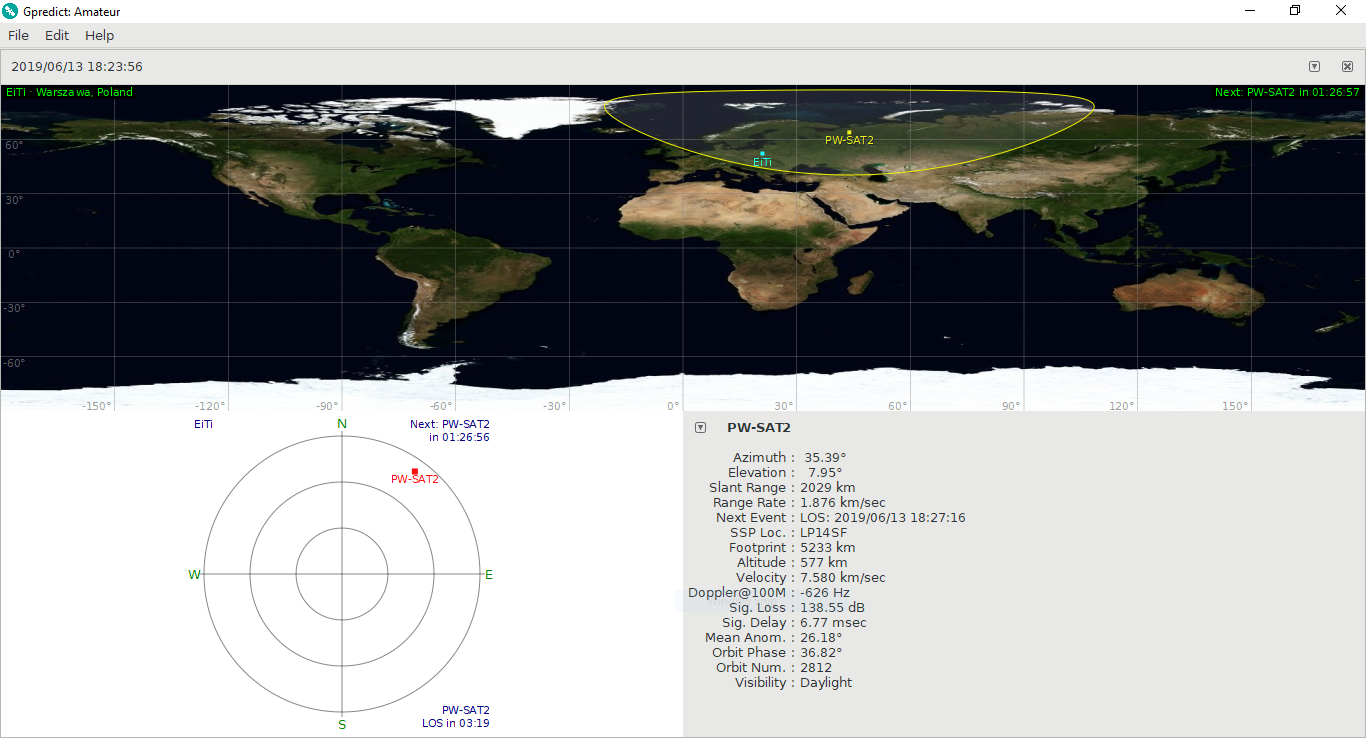
\includegraphics[width=0.8\paperwidth]{img/5/gpredict_pass.png}
    \caption{PW-Sat2 pass in Gpredict software.}
    \label{gpredict_pass}
\end{figure}


\section{Data link budget}
PW-Sat2 have couple of data sources to be sent to the ground, and each of them needs to be taken into account for estimating the required transmission throughput. For each data source the average throughput during ground station coverage is calculated, assuming \SI{30}{\minute} contact per day.
Data to be sent during the primary mission phase (see \ref{sect:mission_phases}):
\begin{itemize}
    \item housekeeping telemetry (satellite health information, such as temperatures, bus and solar panel voltages and currents, subsystem status etc. Telemetry is \SI{230}{\byte} frame and should be transmitted every \SI{1}{\minute} (average \SI{30}{\bps}),
    \item archival housekeeping telemetry (gathered during orbit, when no ground station is in range), telemetry should be downloaded in \SI{5}{\minute} step from the whole operational time, which sums up to \SI{64}{\kilo\byte} per day (average \SI{300}{\bps}),
    \item experiment data, which are started by the operator from the ground and each of them is planned to run once a week (Sun Sensor -  \SI{32}{\kilo\byte}, RadFET - \SI{4}{\kilo\byte}, Cameras (10 photos) - \SI{300}{\kilo\byte}) - it sums up to \SI{336}{\kilo\byte} per week, average of \SI{220}{\bps},
    \item Sail deployment procedure, which transmits experiment data on-line (during the experiment). Estimated data to be transmitted (sail deployment indicator, photos and gyroscopes) is about \SI{1}{\kbps}.
\end{itemize}
During the secondary mission, the satellite is put into deep-sleep mode, and no archival telemetry is archieved and downloaded. The only data sources are periodically executed experiments and photographs of the sail. This reduces the downlink data budget even more.

Data downlink throughput requirement for PW-Sat2 mission sums up to about \SI{1}{\kbps}.
For uplink, the telecommands sent from the ground are relatively short (less than \SI{200}{\byte} each) and the rate of thelecommands is low. Therefore, no specific requirement was created, with minimal usable rate of about \SI{100}{\bps}.

\section{Frequency band selection}



\section{Communication link parameters}
Selected satellite radio module (as described in \autoref{section:comm_design}) imposes the modulation and data packets used in the communication. This section briefly describes used modulations, frame formats and implications to the ground segment of the system.

\subsection{Downlink modulation}
Downlink signal is modulated using Binary Phase Shift Keying (BPSK). The data rate can be changed dynamically by the spacecraft On-Board Computer, in range \si{1.2} - \SI{9.6}{\kbps}, allowing to improve the link quality when necessary. Baseband signal is also filtered using Raised Root Cosine filter, to reduce side lobes power. Signal bandwidth varies between \SI{2.4}{\kHz} (for \SI{1.2}{\kbps}) and \SI{19.2}{\kHz} (for \SI{9.6}{\kbps}).

% TODO: rysunek BPSK

\subsection{Uplink}
Uplink modulation is two-staged: first, data is modulated using Frequency Shift Keying with Bell 202 modem tones (0s and 1s translated to tones \SI{1200}{\hertz} and \SI{2200}{\hertz}), later to be Frequency Modulated on the RF carrier (with frequency deviation of $\pm\SI{5}{\kilo\hertz}$).

% TODO: schemat modulatora

\subsection{Frame format}
Physical layer data format is reduced-functionality AX.25 packet \cite{AX25_standard}. Only connectionless transmission mode and UI frames are supported. Packet framing is the same as in SwissCube CubeSat \cite{SwissCube_AX25}.

Basic frame format is shown in the table \ref{AX25_frame}. All the fields except flags are bit-stuffed to ensure that the \textit{Flag} field does not appear in the data: if there are six '1' bits to be send, transmitter inserts '0' bit before the last one. Adressing in this system in inherent, but unused - this is point-to-point connection, therefore adresses are fixed. Frame-Check Sequence is a CRC (CITT standard) of the whole frame (without \textit{Flags}). \textit{Information Field} is variable-length, between \si{4} and \SI{256}{\byte} length is the place for the actual data transmitted by the On-Board Computer.

\begin{table}
\small
\centering
\caption{AX.25 frame format}
\label{AX25_frame}
\arrayrulecolor{black}
\begin{tabular}{l|c|c|c|c|c|c|c|c|} 
\hhline{~|-|----|-|-|-|}
\multirow{2}{*}{}                                                              & \multirow{2}{*}{Flag } & \multicolumn{4}{c|}{AX.25 Transfer Frame Header (128 bits)}                                                                                                                                                                                   & {\cellcolor[rgb]{0.753,0.753,0.753}}                                                                                                                  & \multirow{2}{*}{\begin{tabular}[c]{@{}c@{}}Frame-\\Check\\Sequence\end{tabular}} & \multirow{2}{*}{Flag}  \\ 
\hhline{~|~|-|-|-|-|>{\arrayrulecolor[rgb]{0.753,0.753,0.753}}->{\arrayrulecolor{black}}|~|~|}
                                                                               &                        & \begin{tabular}[c]{@{}c@{}}Destination\\Address\end{tabular} & \begin{tabular}[c]{@{}c@{}}Source\\Address\end{tabular} & \begin{tabular}[c]{@{}c@{}}Control\\Bits\end{tabular} & \begin{tabular}[c]{@{}c@{}}Protocol\\Identifier\end{tabular} & \multirow{-2}{*}{{\cellcolor[rgb]{0.753,0.753,0.753}}\begin{tabular}[c]{@{}>{\cellcolor[rgb]{0.753,0.753,0.753}}c@{}}Information\\Field\end{tabular}} &                                                                                  &                        \\ 
\hline
\multicolumn{1}{|c|}{\begin{tabular}[c]{@{}c@{}}Length\\{[}bits]\end{tabular}} & 8                      & 56                                                           & 56                                                      & 8                                                     & 8                                                            & {\cellcolor[rgb]{0.753,0.753,0.753}}32-2048                                                                                                           & 16                                                                               & 8                      \\ 
\hline
\multicolumn{1}{|c|}{Value}                                                    & 01111110               & PWSAT2-0                                                     & PWSAT2-0                                                & 00000011                                              & 11110000                                                     & {\cellcolor[rgb]{0.753,0.753,0.753}}                                                                                                                  & CRC-CITT                                                                         & 01111110               \\
\hline
\end{tabular}
\end{table}


Additionally, downlink data is scrambled using G3RUH scrambling polynomial to maximize randomness and ensure proper bit synchronization.
